%!TEX root = ../Main.tex

\chapter{Theory}
This section will describe the theory behind the problem worked with in this project.

\section{Traveling Salesman Problem}
The problem is basically a well-known optimization problem called the Traveling Salesman Problem\cite{wiki:TSP}. The problem consists of creating the shortest route between a set of points, with all points being visited exactly once. 

Given points with 2 coordinates, and assuming "as-the-crow-flies"-movement, the distance between two points is calculated as the euclidean distance between the points. For two points A and B, the distance is calculated as follows:

\begin{equation}
	dist(A,B) = \sqrt{(x_B - x_A)^2 + (y_B - y_A)^2}
\end{equation}

where $x_A$ and $x_B$ are the x-coordinates of points A and B respectively, etc...

The total distance of the route is then calculated as:

\begin{equation}
	dist_{total}(\textbf{points}) = \sum_{i=0}^{N-1}(dist(\textbf{points}(N),\textbf{points}(N+1)))
\end{equation}

where \textbf{points} is a vector of points, in the order they are to be visited and \textbf{points}(N) is the Nth entry in the vector.

The problem is that the number of possible solutions increases with the number of points at a rate of:

\begin{equation}
	nPossibleSolutions=!nPoints
\end{equation}

\label{eq:number_of_possible_solutions}

\begin{figure}[H]
	\centering
	{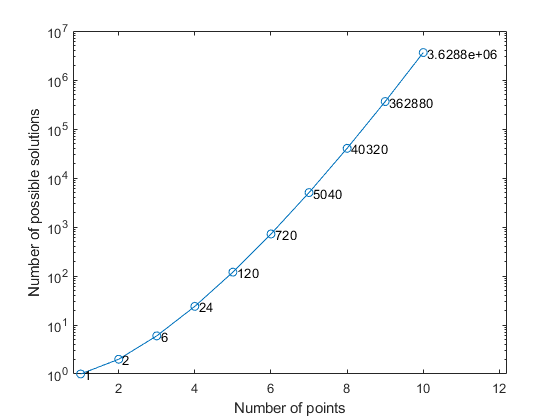
\includegraphics[scale=0.5]{Images/number_of_possible_solutions.PNG}}\\[0.5cm]
	\caption{Number of possible solutions}
	\label{fig:number_of_possible_solutions}
\end{figure}


As the number of possible solutions is equal to the factorial of the number of points, this number quickly increases with an increasing number of points. Thus, optimizing the route by means of brute force (i.e. trying out every single solution) quickly becomes very computationally heavy. In order to avoid optimizing by brute force, global optimization functions can be used in order to find the optimal solution. We have chosen to use the genetic algorithm, as it is easy to implement when doing discrete optimization, which this problem is. Discrete optimization means that there is a finite set of possible solutions, instead of a continuous range of solutions.

\section{Genetic Algorithm}
The genetic algorithm is a meta-heuristic algorithm inspired by the idea of "survival of the fittest". The basic idea is to create a "generation" of sample solutions, by encoding the data of solutions as "chromosomes". New generations of sample solutions are then created by combining these candidate solutions, with the more "fit" samples being more likely to be chosen for "reproduction". The idea is that attributes that result in good fitness will remain, while attributes resulting in bad fitness will be sorted out. Furthermore, each sample has a chance to randomly mutate, which reflects the random mutations happening in nature as well.

For each generation the best solution is found and is compared to the \textit{global} best solution, i.e. the best solution encountered so far over all generations. If the best solution for the generation is better than the global best solution, the global best solution is replaced.

\subsection{Objective function}
In order to evaluate fitness of a sample, an objective function must be implemented. In our case, the objective function is the total route distance, given a certain route of points.

\subsection{Fitness function}
For each sample, the \textit{fitness}, a measure of how good the solution is, is calculated. This measure is used when picking out the candidate solutions used to create a new generation.

In our implementation the fitness of each sample solution will be evaluated as the relative increase or decrease of the objective function for the given sample, compared to the current optimal solution. This is done in order to make the fitness independent of the scaling used to measure distance.

\begin{equation}
	fitness(points) = \frac{dist_{total}(\textbf{points})}{bestFitness_{k-1}}
\end{equation}

where $bestFitness_{k-1}$ is the best fitness score experienced up until last iteration. In the first generation however, the fitness denominator in the fitness-function will be the max of the first generation.

\subsection{Encoding of information}
In order to create combinations of candidate solution, information must be encoded as a \textit{chromosome}. An example could be a candidate solution consisting of a sequence of actions, where each action can be one of two possible actions. This could be encoded as a sequence of binary values.

In our example, the information of each candidate solution is the sequence in which the points are visited. We choose to encode this information as a sequence of letters. For example, one candidate solution is to visit point A, then point E, then point B, then point C. This would be encoded as
A E B C.

\subsection{Creation of new generation}
The creation of a new generation of sample solutions consists of several steps. Two sample solutions from the current generation is selected for \textit{mating} and then two samples in the new generation are created using \text{crossover} and \textit{mutation}.

\subsubsection{Selection of samples for mating}
When creating a new sample solution, two sample solutions in the current generation is picked. When picking sample solutions for mating, the chance of a sample being picked depends on its fitness, with more fit solutions having a larger chance of being picked. Furthermore, it is important that the two picked solutions are not the same, as this would not result in a new sample solution, when doing crossover.

\subsubsection{Crossover}
When two solutions have been picked, two new solutions are created by means of a method called \textit{crossover}. The idea of crossover is to take the chromosome-string from both solutions, "cut" them over at a given point, and then combine the resulting parts to two new solutions. For example, if the data for a solution was encoded as eight binary numbers, crossover could look as follows:

\begin{figure}[h]
	\centering
	{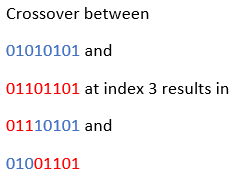
\includegraphics[scale=0.5]{Images/crossover_binary.PNG}}\\[0.5cm]
	\caption{Example of crossover with information encoded as binary numbers}
	\label{fig:crossover_binary}
\end{figure}



In our implementation, crossover is a bit different, seeing that each point can only appear once in a solution. This has been solved, by the following implementation of crossover between solutions A and B at index N:
\begin{enumerate}
	\item The first N elements are taken from solution A.
	\item The first element not filled out is equal to the first element in B not present in the current sample.
	\item Repeat step 2 until all elements are filled out.
\end{enumerate}

where "first" means lowest index in vector. The algorithm is repeated, where solution A and solution B swap places, resulting in 2 new solutions. An example where, information is encoded as letters is:

\begin{figure}[h]
	\centering
	{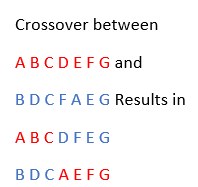
\includegraphics[scale=0.5]{Images/crossover_letters.PNG}}\\[0.5cm]
	\caption{Example of crossover with information encoded as letters}
	\label{fig:crossover_letters}
\end{figure}

\FloatBarrier

\subsubsection{Mutation}
After generating new sample solutions from crossover, there is a chance that each sample solution will mutate, e.g. create a random change to the solution . This chance is decided by a variable mutation rate. In the case of the binary representation of information, mutation could be implemented as a chance for each bit to flip.

In our case, mutation is implemented as a chance to swap the position of two elements of the vector in the sample solution. 

For example:
\begin{figure}[h]
	\centering
	{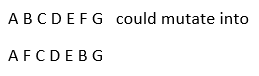
\includegraphics[scale=0.5]{Images/mutation_letters.PNG}}\\[0.5cm]
	\caption{Example of mutation with information encoded as letters}
	\label{fig:mutation_letters}
\end{figure}

\subsection{Stopping criterion}
The algorithm must contain a stopping criterion, which is the criterion that must be fulfilled before the algorithm stops searching for a better solution. Possible stopping criterions are:

\begin{itemize}
	\item Certain number of generations run.
	\item Certain number of generations without improvement in global best solution.
	\item Global best solution evaluates to more/less than certain value.
\end{itemize}

In our case, the stopping criterion will be a certain number of generations without improvement in global best solution. This number has been chosen to be 19, due to implementation details.